\chapter{Diseño experimental y resultados}
En este capítulo se explicarán las decisiones tomadas en cuanto al diseño del experimento con el fin de alcanzar los objetivos previamente mencionados, así como los resultados obtenidos de dicho experimento.
\section{Diseño experimental}
\subsection{Trabajo previo}
En un principio, se quería extraer una base de datos de torques aplicados sobre una sola articulación, manteniendo el resto en una posición fija. A partir de esta base de datos, se diseñaría y entrenaría una red neuronal que aprendiera las posiciones alcanzadas al aplicar una serie de torques durante un intervalo de tiempo. Esta red sería capaz de generar la secuencia de torques a partir de la posición objetivo y la actual, de acuerdo a los datos extraídos en el experimento.

Para ello, en primer lugar se estudiaron las herramientas necesarias para llevar a cabo el proyecto. Estas son: \ros, la API de Baxter y en un principio, el simulador robótico V-REP. Primero se aprendió a usar V-REP, realizando el tutorial que aparece en su manual. Con él se aprendió a realizar un robot con dos ruedas y un sensor de proximidad, capaz de moverse de manera autónoma.

Paralelamente, se estudió \ros haciendo uso del tutorial que ofrece la página web, en el que se aprendió los conceptos de nodo, mensaje, y tema entre otros, así como aprender a usarlos haciendo uso del terminal de linux (bash) y de la librería \textit{rospy}. Se requirió aprender a programar en Python, mientras se aprendían estas otras herramientas.

Una vez estudiados estos temas por separado, se intentó utilizar lo aprendido de \ros sobre la simulación de Baxter que V-REP trae implementada. Desafortunadamente, se descubrió que el simulador no se integraba con \texttt{ROS}, por lo que se estudiaron otros simuladores que sí fueran compatibles.

Se encontró que el propio robot tenía un modelo en el simulador Gazebo, totalmente compatible con los nodos y temas que ejecuta el robot de verdad, y al cual te conectas de la misma manera que lo harías con éste. Por lo tanto, se dedicó un tiempo a estudiar el simulador, aunque ya estaba preparado para probar directamente los experimentos sobre él.

Para familiarizarse con las APIs de Baxter, se realizaron algunos programas que publicaban mensajes a los brazos del robot para controlarlos por posición, velocidad, y torque. También se experimentó con la API de Python y se descubrió en ella una manera mucho más cómoda de comunicarse con el robot.

En las pruebas realizadas, se notó un buen comportamiento del simulador en los controles por posición y velocidad, no así en el control por torques, donde el robot simulado se comportaba sin sentido. Se hizo una versión del controlador PD (sin la componente integradora) que no se comportaba como debía. Dado el comportamiento anómalo del simulador, se decidió probar el programa en el Baxter, descubriendo así el mal funcionamiento del simulador en cuanto a control por torque se refiere.

Una vez familiarizados con el robot y su control, se decide crear un programa que mueva una articulación controlada por torques, mientras que las demás se quedarían quietas (controladas por posición). Desafortunadamente, se descubre que el robot no es capaz de ejecutar este tipo de control híbrido, por lo que es necesario hacer un control por torques del brazo completo. Esto supuso realizar un controlador para las articulaciones que no se mueven. El controlador elegido fue el PID, y tras ajustar los parámetros del mismo haciendo uso del método del ciclo límite, se probó la configuración en el robot.

El controlador no funcionaba como se esperaba, produciendo muchas micro-oscilaciones y oponiendo poca fuerza al intentar mover el brazo, lo que supondría obtener muestras muy ruidosas de la articulación de la cual se deseaba obtener una base de datos. A partir de las constantes anteriores, se intentaron ajustar los parámetro del PID a mano, haciendo uso de un paquete de \ros que implementa el controlador PID y cuyos parámetros se pueden cambiar sobre la marcha. Los resultados mejoraron, pero seguían sin ser satisfactorios.

Se estudiaron técnicas de inteligencia artificial de ajuste de parámetros \cite{wright2015coordinate}\cite{ruge2012aplicacion}, como colonias de hormigas, recocido simulado, o algoritmos genéticos. Se implementó el algoritmo de recocido simulado sobre el PID, calculando el error del mismo como el error absoluto medio ponderado en el tiempo de la posición deseada y las recogidas. Pero las muestras eran muy ruidosas, y una misma configuración de parámetros devolvían errores muy distintos, además que, debido a las grandes fuerzas que aplicaba el robot, éste se paraba durante unos minutos, haciendo inviable el aprendizaje con este tipo de algoritmos, que requiere de miles de iteraciones.

Es por esto por lo que se reestructuró el diseño del problema. Si no se era capaz de encontrar un controlador que mantuviese las articulaciones quietas para realizar el experimento, para así tomar muestras de los torques aplicados sobre una articulación y las posiciones a las que llegaba, se aprendería de todos los torques a la vez.

Una alternativa era realizar el mismo experimento que se quería hacer con una articulación, pero con todas a la vez. El problema era que las fuerzas aplicadas moverían el robot de manera que a priori no se puede predecir su movimiento, lo que hacía que fuera peligroso tanto para las personas que trabajaban con él como para el robot mismo. Además, obtener una base de datos de posiciones a las que llega el robot habiendo aplicados ciertos torques se vuelve infinita, ya que a una misma posición se puede llegar de distintas maneras (desde un mismo sitio) a través de distintos recorridos.

Desechada la idea de controlar por torques el robot para obtener una base de datos, se llega a la conclusión de que la manera más segura y viable, es obtener la base de datos a través del control por posición del propio robot. De esta manera, moveremos el brazo de un lugar a otro y registraremos las posiciones por las que pasa, a la velocidad que lo hace, y los torques aplicados para realizar dicho movimiento.

Se estudia realizar un muestreo de todas las dimensiones del espacio. Se estudia el caso en que a cada dimensión le asignamos dos puntos (los dos extremos de su rango). A continuación, se calcula el número de combinaciones entre todos los puntos de las 7 articulaciones. El resultado es 16256 combinaciones posibles. Suponiendo que cada movimiento tarda de media 2 segundos, y que nunca se realiza el mismo movimiento dos veces, se tardan más de 9 horas en recoger esta base de datos, que solo contiene información para realizar movimientos que van desde los extremos de las articulaciones, a otros extremos. Para tres puntos en vez de dos, el número de combinaciones posibles asciende a 4780782, que supongamos 1 segundo por movimiento (los puntos están más cerca entre sí), son 55 días y 8 horas de toma de datos. Esto sin tener en cuenta que, por motivos de seguridad, no se puede dejar el robot funcionando sin supervisión. La fórmula hallada es la siguiente:

$$ combinaciones = 2 * \sum_{i=1}^{dim^n}(dim^n-i) $$

Donde $dim$ es el número de dimensiones (articulaciones) y $n$ el número de puntos por articulación.

Es por esto por lo que se optó por un enfoque probabilístico, donde las posiciones siguientes a las que se llegaría serían elegidas al azar, eligiendo de manera uniforma las posiciones siguientes para cada una de las articulaciones dentro del rango de cada una, tal y como se explica más adelante.

Una vez estudiados los \hyperref[subsec:metodos/control_baxter]{mecanismos de control del Baxter}, se procedió a extraer una base de datos del control por posición, así como diseñar una red neuronal capaz de aprender de este controlador.

\subsection{Extracción de base de datos}
La base de datos consiste en las posiciones, velocidades y torques registradas por el robot, así como de las órdenes enviadas sobre la posición y la ratio de velocidad deseadas.

Para ello, se hará uso de la \hyperref[subsubsec:metodos/pythonAPI]{interfaz para el lenguaje Python} que ofrece Baxter, así como de la herramienta \hyperref[subsec:metodos/rosbag]{\texttt{rosbag}}.
\subsubsection{Ejecución}
El espacio vectorial de las siete dimensiones formadas por cada una de las articulaciones se muestreará de manera uniforme, a fin de obtener una base de datos representativa del controlador que estamos aprendiendo. Esto significa que, para cada movimiento, se elegirán siete posiciones objetivo (una por articulación) de acuerdo a una distribución uniforme sobre el rango de cada articulación. De igual manera se elegirá una ratio de velocidad objetivo con distribución uniforme entre 0 y 1. El tiempo máximo empleado para cada movimiento será de 15 segundos, tiempo suficiente para permitir el movimiento entre puntos distantes entre sí a una velocidad baja, y por lo tanto, para todos los movimientos.

\subsubsection{Tratamiento}
Una vez obtenida la base de datos, se prepara para la fase de entrenamiento y evaluación de la red neuronal.

\paragraph{Ficheros \texttt{.bag}}
El primer paso consiste en transformar la base de datos en tipos de datos que entienda el lenguaje de programación Python.

Los ficheros obtenidos con \texttt{rosbag} tienen la extensión \texttt{.bag}, y consisten en ficheros conteniendo mensajes sobre los que se iteran. De esta manera, iteramos sobre cada mensaje y leemos su contenido, que consiste en el tema del cual proviene el mensaje, una marca temporal de su recepción por \texttt{rosbag}, y del mensaje en sí mismo.

La marca temporal corresponde al tiempo del reloj interno del ordenador en el cual se recibe el mensaje. Dado que la conexión entre el robot y el ordenador se realiza por tcp/ip, este tiempo diferirá del de generación en el robot. Para paliar con este problema, \texttt{ROS} dispone una marca temporal dentro del cuerpo del mensaje con el instante de creación del mensaje en el robot (de acuerdo a su reloj interno), además de un número de secuencia para ordenar los mensajes en el ordenador.

\subparagraph{Error en frecuencia}
Gracias a esta información, se percibió un error en frecuencia entre el reloj del ordenador y el del robot. Esto significa que, a una frecuencia de generación de mensajes de 100 Hz, el ordenador generó 100 posiciones y velocidades deseadas por segundo (suponiendo que es el que tiene el reloj ajustado correctamente), mientras que el robot generó 99 posiciones, velocidades y torques actuales. Para solventar este problema, en primera instancia se representó gráficamente la diferencia de mensajes obtenidos por parte del ordenador y el robot en función del tiempo (figura \ref{fig:resultados/diferencia}).

\begin{figure}[]
	\centering
	\begin{subfigure}[b]{0.45\textwidth}
		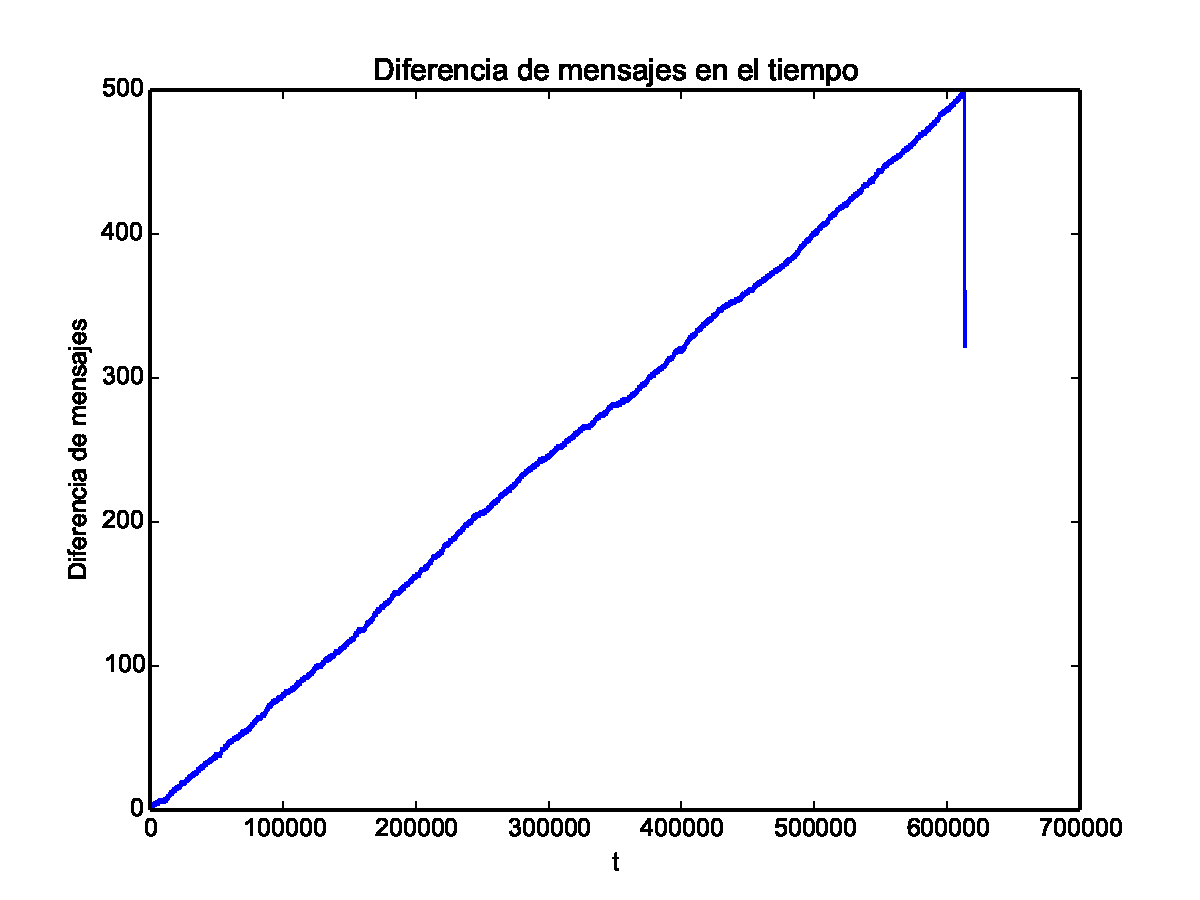
\includegraphics[width=\linewidth]{imagenes/resultados/diferencia.pdf}
		\caption{Señal sin procesar}
		\label{fig:resultados/diferencia}
	\end{subfigure}
	\begin{subfigure}[b]{0.45\textwidth}
		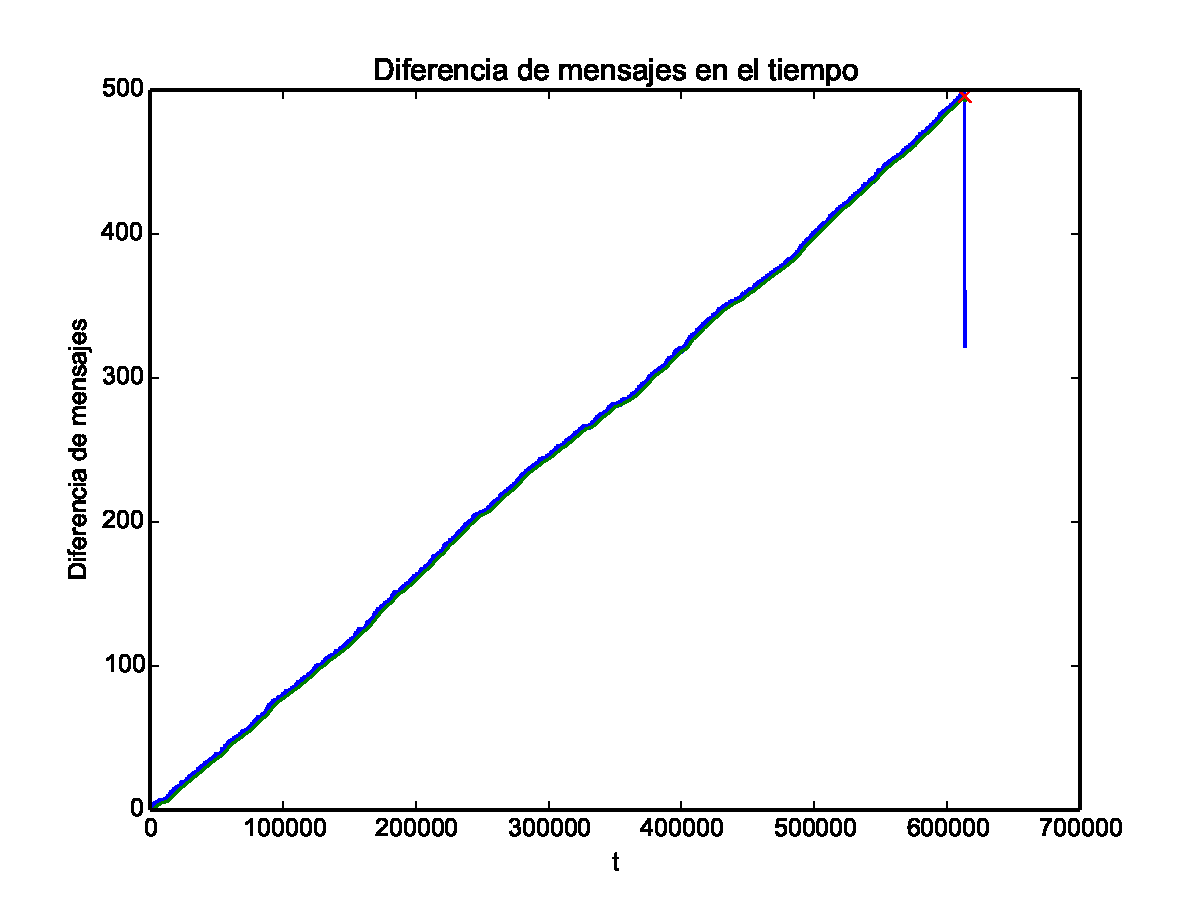
\includegraphics[width=\linewidth]{imagenes/resultados/diferenciafilt.pdf}
		\caption{Señal filtrada paso baja}
		\label{fig:resultados/diferenciafilt}
	\end{subfigure}
	\caption{Diferencia de mensajes recibidos del ordenador y del robot}
\end{figure}

Como se puede observar, esta diferencia crece con el tiempo, lo que significa que el ordenador genera mensajes a mayor velocidad que el robot. Es cuando el ordenador deja de generar mensajes cuando esta diferencia cae en picado, momento en el cual, los mensajes generados por el robot dejarán de corresponderse con las posiciones deseadas y pasarán a corresponderse con las posiciones, velocidades y torques del robot manteniendo la última posición alcanzada.

Por lo tanto, el objetivo será encontrar el momento en el que ocurre dicha bajada, es decir, el pico. El problema surge cuando la señal no es monótona, sino que, como se observa en la figura \ref{fig:resultados/diferenciadetalle}, crece y decrece en intervalos temporales pequeños (debido a la naturaleza a ráfagas de la señal). Para paliar con este inconveniente, se realiza un filtrado paso baja (con un filtro de media móvil) que elimine dicha componente frecuencial. El resultado es el que se observa en las figuras \ref{fig:resultados/diferenciafilt} y \ref{fig:resultados/diferenciadetallefilt}. A partir de esta señal, solo queda seleccionar el valor máximo de la misma. El valor obtenido es el número de mensaje recibido hasta el cual los mensajes son válidos.

\begin{figure}[]
	\centering
	\begin{subfigure}[b]{0.45\textwidth}
		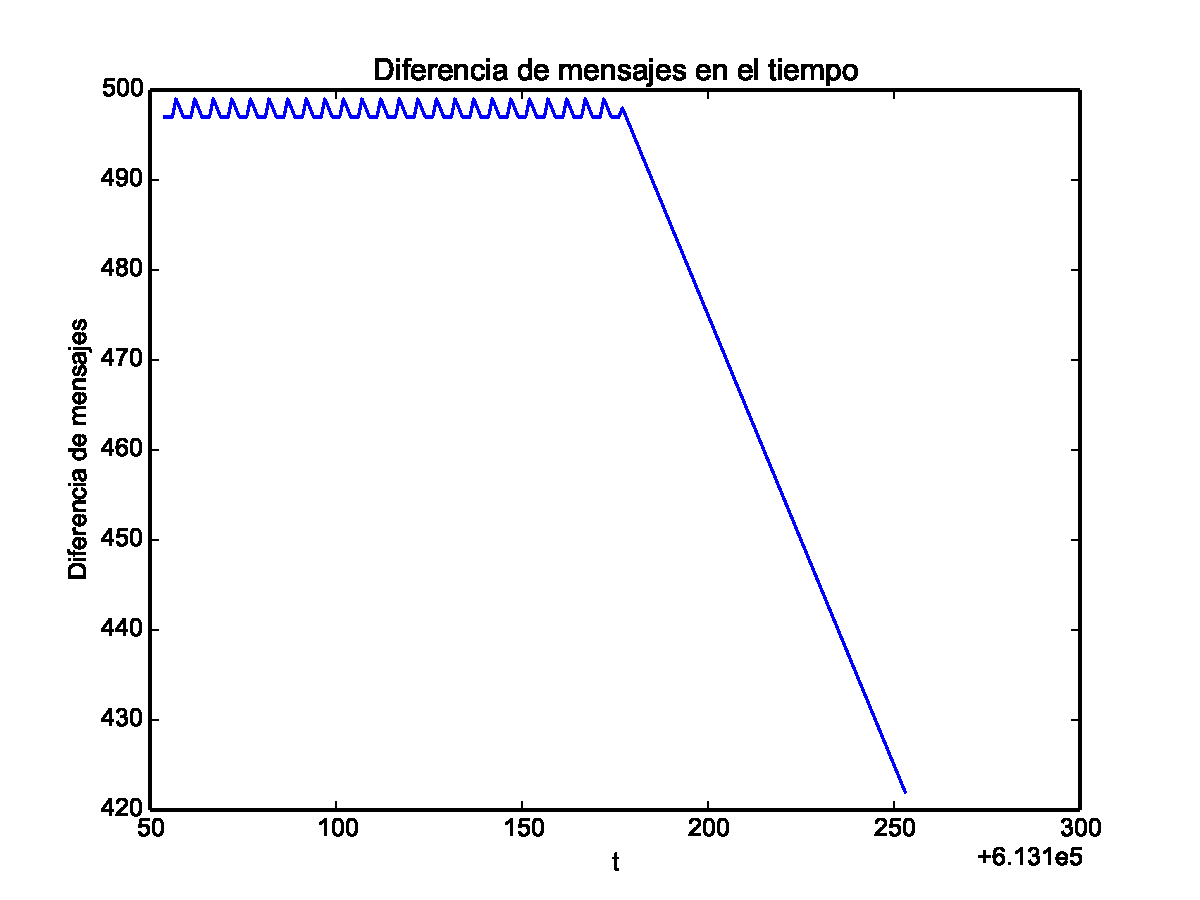
\includegraphics[width=\linewidth]{imagenes/resultados/diferenciadetalle.pdf}
		\caption{Señal sin procesar}
		\label{fig:resultados/diferenciadetalle}
	\end{subfigure}
	\begin{subfigure}[b]{0.45\textwidth}
		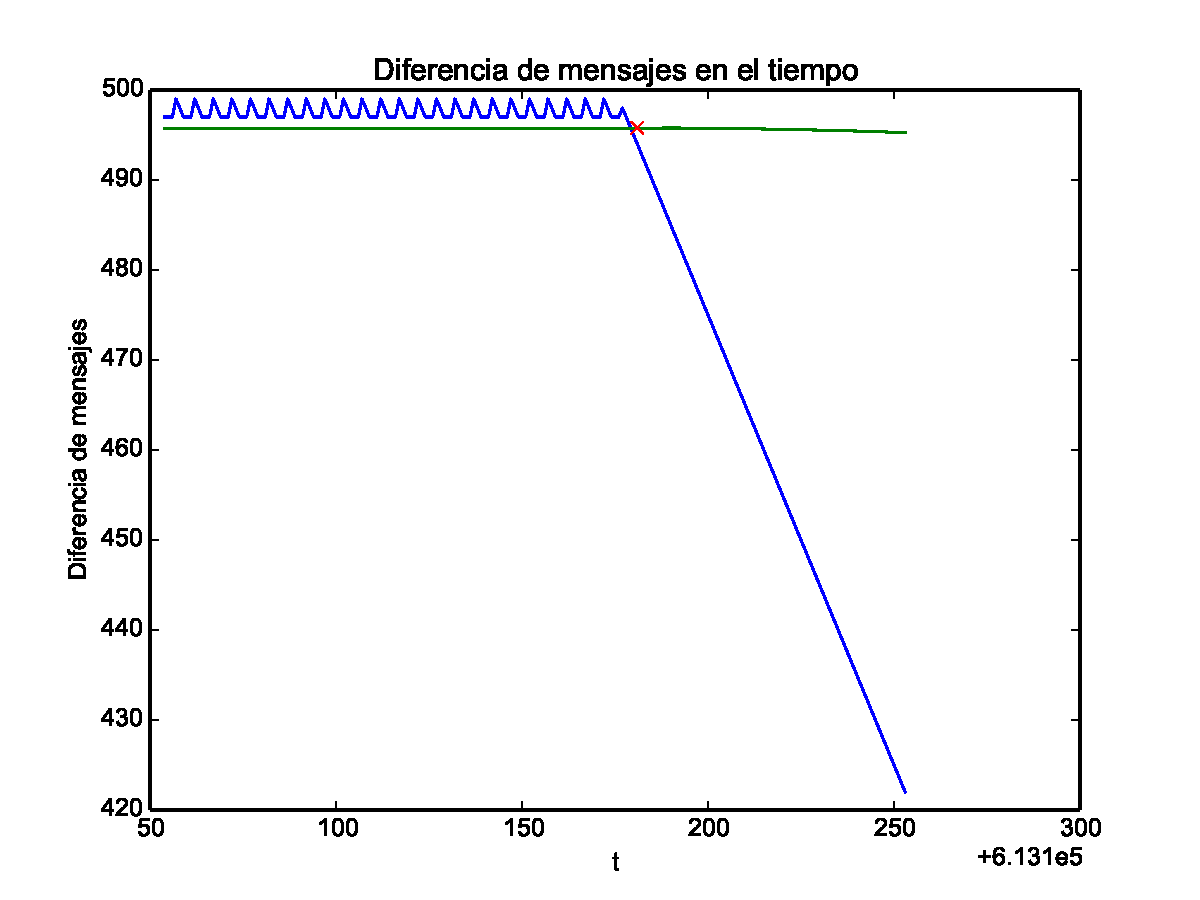
\includegraphics[width=\linewidth]{imagenes/resultados/diferenciafiltdetalle.pdf}
		\caption{Señal filtrada paso baja}
		\label{fig:resultados/diferenciadetallefilt}
	\end{subfigure}
	\caption{Detalle de diferencia de mensajes recibidos del ordenador y del robot}
\end{figure}

Dado que el control lo vamos a realizar desde el ordenador, adaptamos los mensajes recibidos al mismo. Esto lo hacemos mediante interpolación lineal en las posiciones, velocidades y torques recibidos.

De esta manera, se obtienen vectores de la misma longitud (en el tiempo) tanto enviados como recibidos.

\subparagraph{Ráfagas}
También se percibió la llegada a ráfagas en los mensajes provenientes del robot. Esto no supone un problema para preparar los datos, pero sí lo es a la hora de realizar un controlador realimentado que requiere la información que proporciona el robot sin desfases. El controlador propuesto en este trabajo no es realimentado, pero de serlo, una posible solución sería implementar el controlador en el propio robot (no ejecutarlo en el ordenador), aunque para ello habría que tomar nuevamente la base de datos o ajustarla a la frecuencia de generación de mensajes del robot. Otra posible solución consistiría en un predictor de posiciones y velocidades que ofrezcan al controlador esta información cuando no disponga de la misma. Por ejemplo, supongamos que en un instante concreto, llega una ráfaga de tres posiciones, velocidades y torques provenientes del robot. Esto significa que, dos instantes anteriores, el ordenador no ha obtenido ninguna información, por lo que la última posición, velocidad y torques conocidos son los obtenidos hace dos instantes temporales. En este caso, el predictor generaría 2 posiciones y velocidades (los torques serían la salida del sistema) para los instantes temporales que no disponen de información directa.


\subsection{Red Neuronal}
A continuación se estudia la viabilidad de la implementación de un controlador a partir del propio de Baxter basado en redes neuronales de aprendizaje profundo.
\subsubsection{Viabilidad}
El primer problema a enfrentarse es el de demostrar que la red neuronal es capaz de aprender algo de los datos extraídos del controlador del Baxter. Por la capacidad de detectar colisiones sabemos que es un sistema realimentado, posiblemente con un controlador PID.

Se podría realizar un controlador donde el modelo dinámico (controlador anticipativo) fuera desempeñado por la red neuronal, y donde la realimentación fuera desempeñada por el controlador PID. También podría implementarse la realimentación como otra red neuronal, pero ambas aproximaciones tienen el problema de enfrentarse a la realimentación y al tiempo real (a una frecuencia de realimentación de 100 Hz). Las redes neuronales profundas tienen el problema de ser pesadas en el cómputo (debido a las no linealidades usadas para la activación de las neuronas), poniendo en riesgo la capacidad de afrontar el problema en tiempo real.

Es por esto por lo que se decide hacer un controlador sin realimentación, donde los datos de entrada sean posiciones objetivo, posiciones en el momento de iniciar el movimiento, y velocidad objetivo, siendo los de salida una sucesión de torques a aplicar para alcanzar la posición deseada.

Para ello se elige una arquitectura basada en redes neuronales realimentadas, ya que las no realimentadas tienen la limitación de generar la misma salida ante la misma entrada, y siendo nuestra entrada única (debido a que el sistema no es realimentado), generaríamos siempre la misma salida, en vez de la sucesión de torques deseada.

Nos encontramos con el problema de si un modelo no realimentado, puede aprender del implementado por Baxter, que sí lo es. El controlador del Baxter consiste en un controlador mixto, formado por uno realimentado y otro anticipativo.

El controlador realimentado no es más que un sistema (lineal o no) que a ciertas entradas genera ciertas salidas (en función de su historia o no). El controlador anticipativo igualmente es un sistema que tiene en cuenta el modelo dinámico del robot, y por lo tanto los dos sistemas son reproducibles por una red neuronal. Por último, tenemos la realimentación, y es en este aspecto, donde la red neuronal tendrá que aprender a producir estimaciones de la salida provocada (posiciones de las articulaciones) al aplicar los torques.

Por lo tanto, la viabilidad de nuestro controlador depende de la capacidad de la red para generar dicha estimación de la realimentación.

Es por ello por lo que se utilizarán redes neuronales recurrentes, ya que tanto el controlador realimentado, como el anticipativo, como la realimentación en sí misma son sistemas que dependen de la historia de las señales de las que dependen, y esto es exactamente lo que hacen este tipo de redes.

\subsubsection{Diseño}
El diseño de la red se ha realizado haciendo uso de la librería \textit{Keras}, que ofrece una capa de abstracción de diseño de redes profundas sobre \textit{Tensorflow}.

El diseño consiste en las siguientes capas, una a continuación de la siguiente:

\begin{enumerate}
	\item Capa de entrada. Esta capa aceptará matrices de $n$x15, donde $n$ es la cantidad de datos a procesar en cada grupo de entrenamiento, y 15 es el número de dimensiones de entrada (7 de las posiciones deseadas, 7 de las posiciones de inicio, y 1 de la ratio de velocidad deseada).
	\item Capa de repetición de vector. La entrada consiste en un único conjunto de datos. Sin embargo, se desea obtener una salida con tantos instantes temporales como longitud tenga la secuencia de mayor tamaño, por lo que repetimos el vector de entrada en el tiempo.
	\item Capa totalmente conectada. La entrada se enlaza con una capa de 64 neuronas con activación relu.
	\item Dropout. Se realiza una selección de neuronas aleatoriamente haciendo uso de la técnica de dropout, para así regularizar la salida.
	\item GRU. El número de capas, así como el número de neuronas variará en función del experimento que se esté realizando. La activación es relu, y cuenta con mecanismos de dropout entre las conexiones recurrentes, así como regularización L1 y L2.
	\item Dropout.
	\item (Capa de convolución 1D + Dropout). Esta capa se activará o desactivará en función del experimento que se realice.
	\item 2 capas totalmente interconectadas. De 500 neuronas cada una y activación relu
	\item Dropout.
	\item Capa de salida (totalmente interconectada). De tamaño 22 (7 de torque, 7 de posición, 7 de velocidad, y 1 de la máscara).
\end{enumerate}

Se ha elegido GRU en vez de las celdas LSTM porque requiere de un menor cómputo, y permite hacer más iteraciones en la misma cantidad de tiempo, ofreciendo resultados similares.

La capa de convolucion 1D es un tipo de capa que opera sobre subconjuntos agrupados de entradas. Sirven para extraer dependencias espaciales en el conjunto de datos.

En la capa de salida, se han añadido las posiciones y velocidades obtenidas en cada momento, a fin de que el error generado por las mismas ayude a la red a aprender. Esto se ha realizado porque existe una dependencia entre los torques generados y la velocidad y posición que el brazo obtiene en cada momento. Los valores que realmente nos interesan son los de torque y máscara, por lo que se ha ponderado la aportación de las posiciones y velocidades por 0.1.

La capa de máscara sirve para delimitar la cantidad de torques válidos en cada secuencia. Esta capa es necesaria, ya que cada movimiento es de una longitud temporal distinta. Una vez entrenada la red generaremos torques de longitud variable, y sabremos qué cantidad de esos torque utilizar gracias a esta máscara.

En la fase de compilación del modelo, se ha elegido el optimizador Adam, y el tipo de error empleado ha sido el error absoluto promedio para los torques, y la entropía cruzada para la máscara (que representa la probabilidad de que el torque actual forme parte del movimiento necesario para alcanzar la posición deseada).

\subsubsection{Experimentos}
Una parte importante en el aprendizaje automático es la modificación y elección de parámetros (como la cantidad de capas, de neuronas por capa, la aportación al error de los métodos de regularización L1 y L2, así como la probabilidad de desactivar una neurona por el método dropout).

Para ello, se dividen los datos en 3:

\begin{itemize}
	\item Conjunto de entrenamiento. Utilizado para entrenar la red.
	\item Conjunto de validación. Para obtener una medida del error de la red para cada uno de los parámetro a modificar.
	\item Conjunto de test. Para obtener una medida independiente de la elección del modelo y los parámetros que indique la eficacia de la red.
\end{itemize}

El problema de dividir en conjunto de entrenamiento y de validación, es que el error obtenido en el conjunto de validación depende del propio conjunto, y por lo tanto no es una medida totalmente fiable para seleccionar los parámetros. Es por esto por lo que se utiliza la técnica de K-pliegues (K-folding). Esta técnica consiste en realizar la división de un único conjunto (además del conjunto de test) en $k$ subconjuntos. Después se realizará el entrenamiento de la red con todos menos con el un conjunto, y se medirá el error de la red sobre este conjunto. El entrenamiento se realiza excluyendo cada vez un subconjunto diferente (y añadiendo el anterior al conjunto de entrenamiento). Al final del proceso, obtendremos un erro medio, así como una desviación típica de la misma.

En base a los datos obtenidos con este método, se elegirá la red que mejores resultados ofrezca, y se medirá su error sobre el conjunto de test.

Los parámetros probados son:

\begin{itemize}
	\item GRU.
	\begin{itemize}
		\item 2 capas de 100 neuronas cada una.
		\item 1 capa de 1000 neuronas.
	\end{itemize}
	\item Regularización L1/L2.
	\begin{itemize}
		\item L1 ó L2 con nivel de regularización 1e-6.
		\item L1 ó L2 con nivel de regularización 0.001.
	\end{itemize}
	\item Dropout.
	\begin{itemize}
		\item Probabilidad de anular la neurona: 0.3.
		\item Probabilidad de anular la neurona: 0.5.
		\item Probabilidad de anular la neurona: 0.6.
		\item Probabilidad de anular la neurona: 0.8.
	\end{itemize}
	\item Convolución 1D.
	\begin{itemize}
		\item Activada.
		\item Desactivada.
	\end{itemize}
\end{itemize}
\subsubsection{Preparación de los datos}
Para entrenar la red, hace falta preparar los datos. Esta preparación consiste en dividirlos  en movimientos, normalizarlos (para un entrenamiento más rápido y robusto de la red), e igualar la longitud de las secuencias, ya que Keras necesita que todos los subgrupos que se utilicen para entrenar la red tengan la misma longitud.

También se creará la máscara, que valdrá 1 para todos los valores de torque que no se hayan puesto a 0, y 0 para los valores de relleno. Se utilizará esta máscara para el cálculo del error, ya que de no hacerlo, la red tendría en cuenta los errores cometidos en la sección de relleno.

\section{Resultados}
A continuación se muestran los resultados obtenidos de la anterior experimentación.
\subsection{Base de datos}
Por motivos de tiempo de entrenamiento, así como para aislar potenciales problemas a la hora de realizar el entrenamiento, se han tomado distintas bases de datos.

\begin{itemize}
\item [Todas las articulaciones] El grueso de nuestra base de datos se ha realizado a partir del movimiento de todas las articulaciones, a distintas velocidades, con un tiempo de espera de 15 segundos.
\item [Una articulación] Se ha aislado el problema del tamaño del espacio a muestrear (las siete articulaciones, cada una con su rango de movimiento) reduciéndolo a una de las siete articulaciones en todo su rango de movimiento. El resto de las articulaciones se mantienen quietas en la posición cero.
\item [5 segundos] En lugar de limitar el tiempo para cada movimiento a 15 segundos, se limita a 5 segundos, para así aislar el problema de desdoblar la red en un intervalo de tiempo tan alto 
($\SI{15}{\second} * \SI{100}{\hertz} = \SI{1500}{muestras}$).
\item [0.5 seg. ratio vel. 1] Es el caso más simple para entrenar la red. Se mueve una sola articulación (el resto se ubican en la posición 0) a máxima velocidad (relación de velocidad 1) durante 0.5 segundos. De esta manera obtenemos una base de datos muy amplia (más de 120 posiciones objetivo por minuto) con el problema del tamaño del espacio y del desdoblamiento temporal muy limitados.
\end{itemize}

Adicionalmente, se ha obtenido un conjunto de datos con combinaciones de distintas articulaciones, así como del brazo con las pinzas anexas para un tiempo máximo de 15 segundos y velocidad variable.

El tamaño total de la base de datos sin procesar es de 5 GB. A una velocidad de generación media de 94 KB/s, es un total de quince horas y media de recogida de datos.

\subsection{Red neuronal}
Se realizaron los experimentos descritos sobre la red neuronal. Por motivos de tiempo de entrenamiento, así como de obtención de la base de datos, se ha realizado el experimento con el conjunto de datos de 0.5 segundos por movimiento (unas 50 muestras por movimiento) y ratio de velocidad 1, esto es, a velocidad máxima.

Los resultados de todos los experimentos son los que se muestran en las figuras \ref{fig:resultados/torque_all}, \ref{fig:resultados/mask_all} y \ref{fig:resultados/all}. Estas gráficas se han obtenido haciendo uso del programa \textit{tensorboard}.

En el eje horizontal se muestra el tiempo relativo durante el entrenamiento, mientras que en el eje vertical se observa el error. Observamos el error cometido durante la fase de entrenamiento de las redes neuronales descritas con anterioridad.

Por motivos de espacio, no se muestran todas las gráficas para cada una de las configuraciones. En su lugar, se muestran las gráficas con los resultados de todas las redes y se explican los comportamientos de cada una de las redes, y por qué se comportan como se comportan en el entrenamiento.

\subsubsection{Error en el torque}
Como se observa en la figura \ref{fig:resultados/torque_loss_all}, el error de entrenamiento es muy grande para algunas configuraciones de la red. Estas configuraciones corresponden con los modelos con un nivel de dropout de 0.8. Este nivel tan alto provoca en el entrenamiento que la salida no tenga nada que ver con la salida que generaría la red de no anularse las neuronas, y ésto es lo que hace que el error de entrenamiento sea tan alto.

Es la misma configuración la que en el conjunto de validación (fig. \ref{fig:resultados/val_torque_loss_all}) devuelve valores constante en torno a 0.76. Esto significa que la red está siendo infrautilizada, y no está aprendiendo. Lo mismo ocurre para la configuración de dropout igual a 0.6 y los valores de regularización L1 de 0.001 y de 1e-6. Los motivos del nivel de dropout a 0.6 son los mismos que para el nivel 0.8, mientras que el motivo por el cual la regularización L1 no funciona como se espera es que, en este caso, el tener neuronas especializadas a costa de apagar otras no funciona.

\begin{figure}[thb]
	\begin{subfigure}[b]{0.45\textwidth}
		\centering
		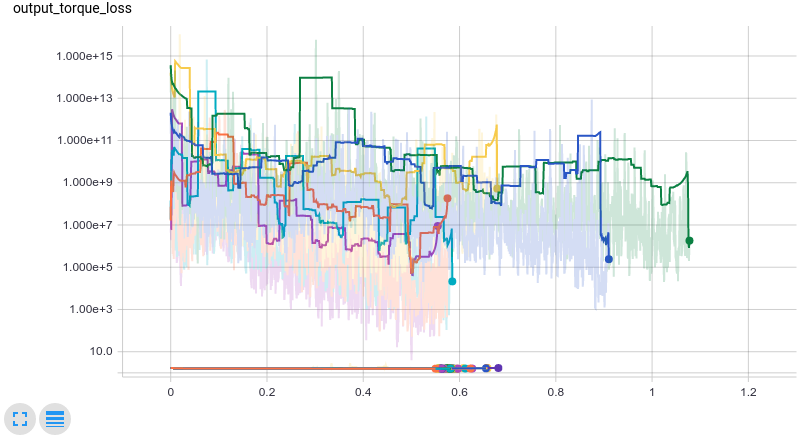
\includegraphics[width=\linewidth]{imagenes/resultados/torque_loss_all.png}
		\caption{Entrenamiento}
		\label{fig:resultados/torque_loss_all}
	\end{subfigure}
	\begin{subfigure}[b]{0.45\textwidth}
		\centering
		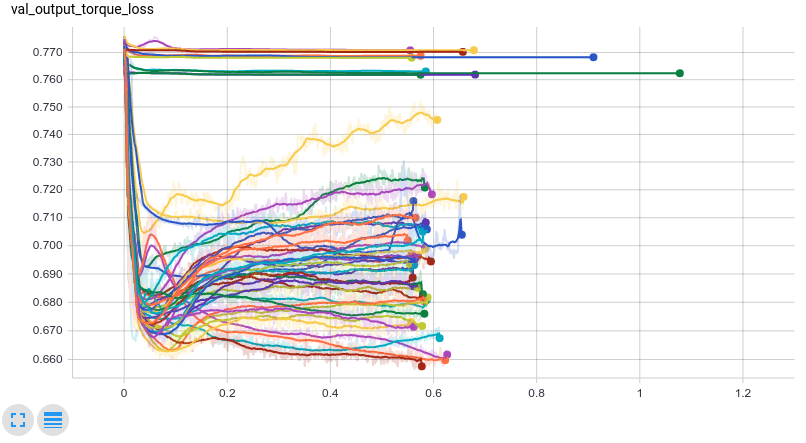
\includegraphics[width=\linewidth]{imagenes/resultados/val_torque_loss_all.png}
		\caption{Validación}
		\label{fig:resultados/val_torque_loss_all}
	\end{subfigure}
	\caption{Errores en el torque}
	\label{fig:resultados/torque_all}
\end{figure}

El resto de redes se comportan de manera similar en cuanto a torque se refiere. Las que mejor resultado dan son las que usan un nivel de regularización L2 de 0.001, 1000 neuronas y 1 capa, y un nivel de dropout de 0.5. Las redes de 2 capas y 100 neuronas no funcionan tan bien como las de 1 y 1000, debido a que las conexiones a través del tiempo de las celdas GRU está generando un fenómeno de sobre-aprendizaje sobre la base de datos de entrenamiento. Esto significa que está aprendiendo a reproducir los patrones de ruido temporales de las señales de entrenamiento.

Por otro lado, el nivel de regularización L2 de 1e-6 parece insuficiente para evitar este sobre-aprendizaje de la red. El sobre-aprendizaje se observa en que la curva de aprendizaje para el conjunto de entrenamiento sigue bajando, mientras que en el conjunto de validación, sube, lo que significa que sigue aprendiendo de la base de entrenamiento, pero lo aprendido no mejora (e incluso empeora) los resultados en datos no vistos antes.

También se observa que, aunque está aprendiendo, el error es muy grande (en torno a 0.7). Hay que recordar que la salida está normalizada, por lo que tiene media 0 y desviación típica 1. Por lo que un error de estas dimensiones significaría que no está aprendiendo casi nada.

En realidad, lo que está ocurriendo es que la mayoría de articulaciones (todas menos una) se mantienen quietas, por lo que el rango de torques que están aplicando es mínimos. Esto provoca que, al normalizarlos, se amplifique en gran escala el ruido de los sensores al leer el torque (que tendría que ser para algunas articulaciones prácticamente constante). El problema es que el error generado por ese ruido afecta al error total igual que las articulaciones que sí tienen un rango más grande de operación y cuya relación señal ruido es mucho menor.

Este problema, una vez conocido, no debe preocuparnos, ya que las redes buscan patrones, y el ruido es la ausencia de dichos patrones, por lo que el aprendizaje no se verá afectado de manera tan negativa como parece en las gráficas.

\subsubsection{Error en la máscara}

Este fenómeno de sobre-aprendizaje es especialmente notable en la salida de la máscara (fig. \ref{fig:resultados/mask_all}). En ella se observa cómo, en el conjunto de entrenamiento, el error baja hasta niveles cercanos a 0, mientras que en la validación estos errores crecen por encima de 0.5. Estos errores tan altos en la máscara se deben a que realmente no hay una relación entre la entrada y la máscara en la base de datos elegidas (1 articulación moviéndose a máxima velocidad durante 0.5 segundos), sino que la máscara depende de la precisión con la que se generaban los mensajes en el Baxter, ya que los movimientos nunca llegan a la posición destino con velocidad 0 (condición para empezar el siguiente movimiento), sino que agotan todo el tiempo en intentar llegar a la posición objetivo. Esto hace que la máscara tome valores de 50 y 51 para la mayoría de muestras, siendo así una medida independiente de la señal de entrada, y por lo tanto no la pueda aprender la red.

Es por esto por lo que se decide no tener en cuenta las medidas del error que la máscara genera, y centrar toda la atención en los errores generados por el torque.

\begin{figure}[thb]
	\begin{subfigure}[b]{0.45\textwidth}
		\centering
		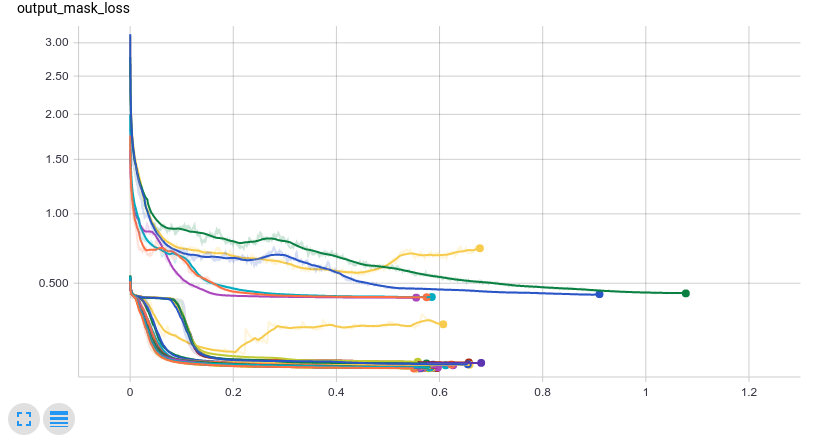
\includegraphics[width=\linewidth]{imagenes/resultados/mask_loss_all.png}
		\caption{Entrenamiento}
		\label{fig:resultados/mask_loss_all}
	\end{subfigure}
	\begin{subfigure}[b]{0.45\textwidth}
		\centering
		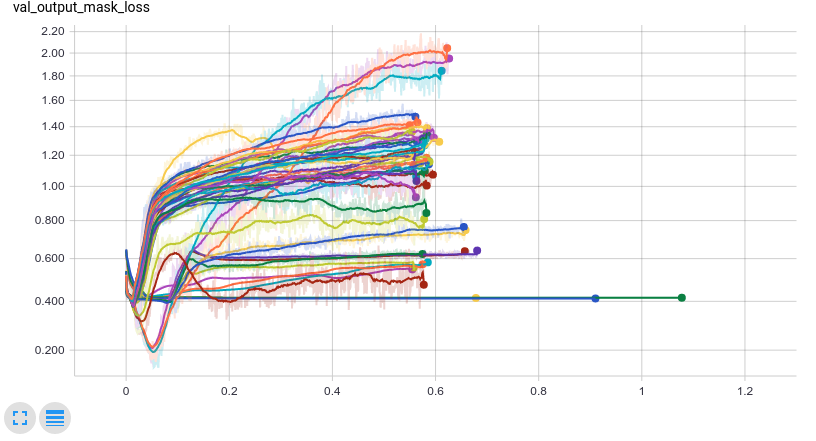
\includegraphics[width=\linewidth]{imagenes/resultados/val_mask_loss_all.png}
		\caption{Validación}
		\label{fig:resultados/val_mask_loss_all}
	\end{subfigure}
	\caption{Errores en la máscara}
	\label{fig:resultados/mask_all}
\end{figure}

\subsubsection{Error total}
El error total (fig. \ref{fig:resultados/all}) es la suma ponderada de los errores cometidos en los torques, la máscara, la posición y la velocidad. Los dos primeros suman al error multiplicados por 1, mientras que los otros dos multiplican por 0.1. Debido a que el objetivo de la red neuronal es obtener unos torques y una máscara adecuada, se han omitido las gráficas de las otras dos fuentes de errores.

\begin{figure}[thb]
	\begin{subfigure}[b]{0.45\textwidth}
		\centering
		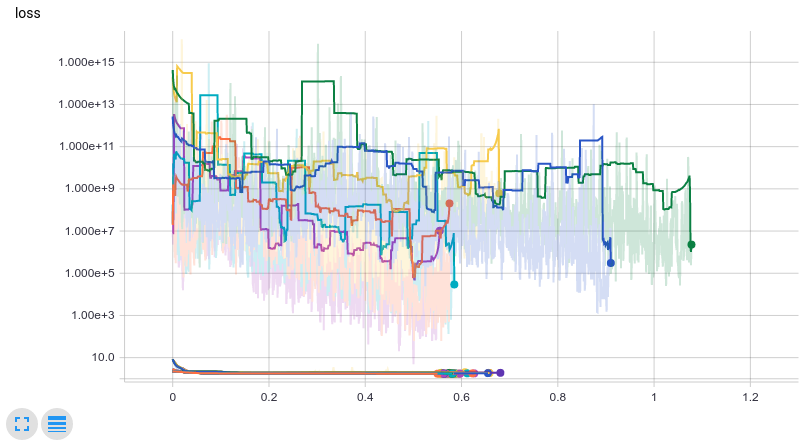
\includegraphics[width=\linewidth]{imagenes/resultados/loss_all.png}
		\caption{Entrenamiento}
		\label{fig:resultados/loss_all}
	\end{subfigure}
	\begin{subfigure}[b]{0.45\textwidth}
		\centering
		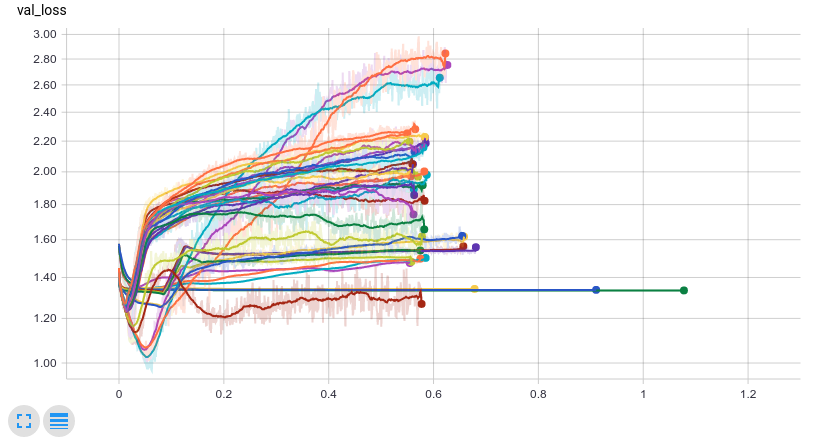
\includegraphics[width=\linewidth]{imagenes/resultados/val_loss_all.png}
		\caption{Validación}
		\label{fig:resultados/val_loss_all}
	\end{subfigure}
	\caption{Errores totales}
	\label{fig:resultados/all}
\end{figure}

\subsubsection{Comparación de torques generados}
En la figura \ref{fig:resultados/final} se muestran los errores de entrenamiento y validación para cada uno de los subconjuntos usando la técnica de k-fold. La red neuronal elegida es la dicha anteriormente: 1 capa y 1000 neuronas, valor de regularización L2 0.001, dropout 0.5, sin capa convolucional ni error L1.

\begin{figure}[]
	\begin{subfigure}{0.45\textwidth}
		\centering
		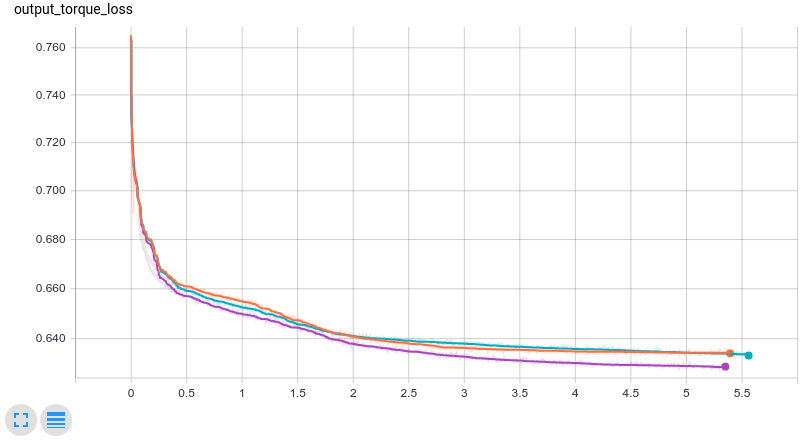
\includegraphics[width=\linewidth]{imagenes/resultados/torque_final.png}
		\caption{Entrenamiento}
		\label{fig:resultados/torque_final}
	\end{subfigure}
	\begin{subfigure}{0.45\textwidth}
		\centering
		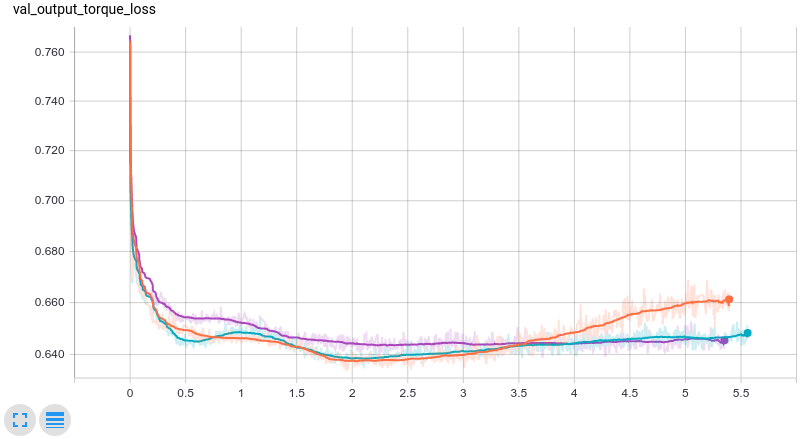
\includegraphics[width=\linewidth]{imagenes/resultados/val_torque_final.png}
		\caption{Validación}
		\label{fig:resultados/val_torque_final}
	\end{subfigure}
	\caption{Errores en el torque}
	\label{fig:resultados/final}
\end{figure}

Debido a que se detectó que los movimientos no acababan (la razón por la que la máscara no se podía aprender, y la mayoría de secuencias tenía una longitud de 50-51 muestras), se decide incluir la velocidad inicial del movimiento, ya que, si no termina el movimiento, significa que lleva una velocidad asociada, por lo que mejoraremos el rendimiento de la red al introducir esta información que antes suponíamos nula (velocidad 0 en todas las articulaciones).

Se observa que la red aprende adecuadamente a extraer los patrones de la base de datos (error decreciente con el número de iteraciones). Además, se observa que se ha conseguido disminuir el efecto del sobre-aprendizaje, ya que el error de validación apenas crece una vez alcanzado el mínimo, y que el error de entrenamiento es comparable al de validación.


En la figura \ref{fig:resultados/pred} se observan las predicciones que realiza la red. Se observa que la red es capaz de seguir la tendencia de baja frecuencia de cada una de las articulaciones. Se observa que, en articulaciones como la s0, donde el rango de operación es muy pequeño, la red ignora las perturbaciones (ruido) y sigue la tendencia general.


En las articulaciones donde el rango es mayor, esto también es cierto. Además, en estas últimas, se observa que las saltos grandes no los sigue. Estos cambios bruscos de torque se corresponden con la aportación que hace el controlador realimentado, y depende de una señal externa, y por lo tanto, incorrelada con el sistema que se pretende controlar. Es por esto por lo que la red no es capaz de aprender dichos cambios.

\begin{figure}[hbt]
	\begin{subfigure}{0.3\textwidth}
		\centering
		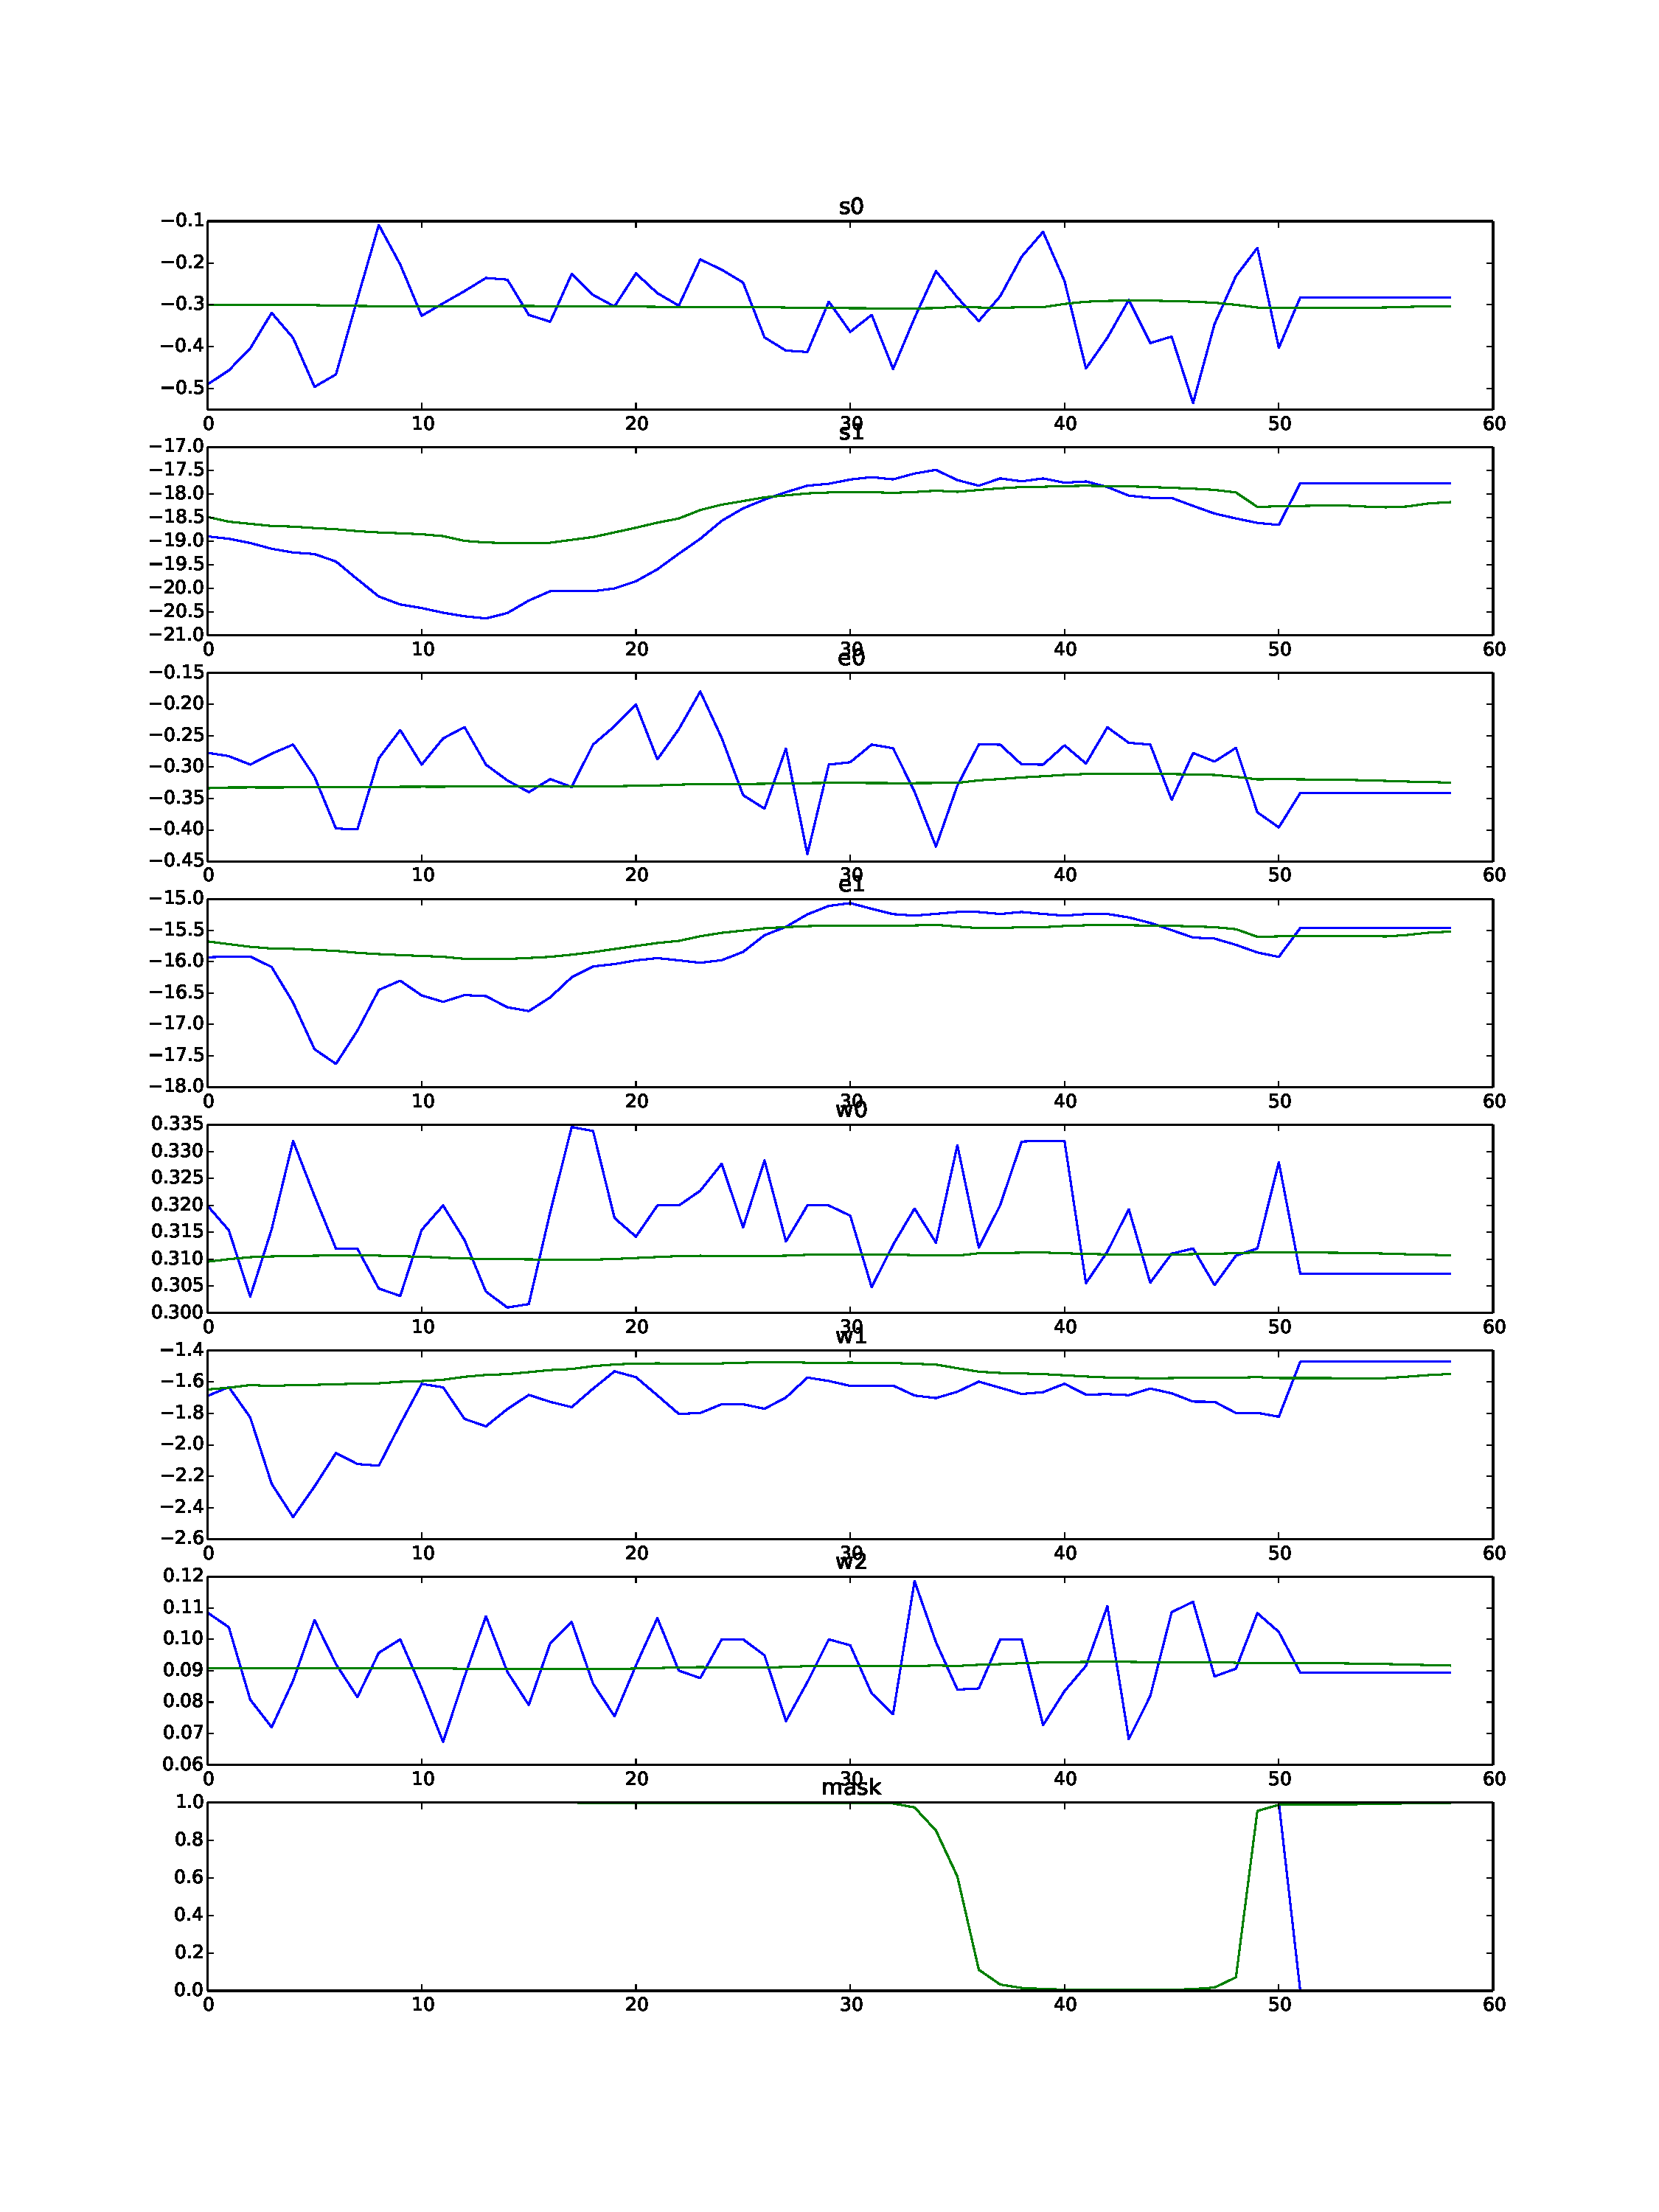
\includegraphics[width=\linewidth]{imagenes/resultados/pred_train.pdf}
		\caption{Entrenamiento}
		\label{fig:resultados/pred_train}
	\end{subfigure}
	\begin{subfigure}{0.3\textwidth}
		\centering
		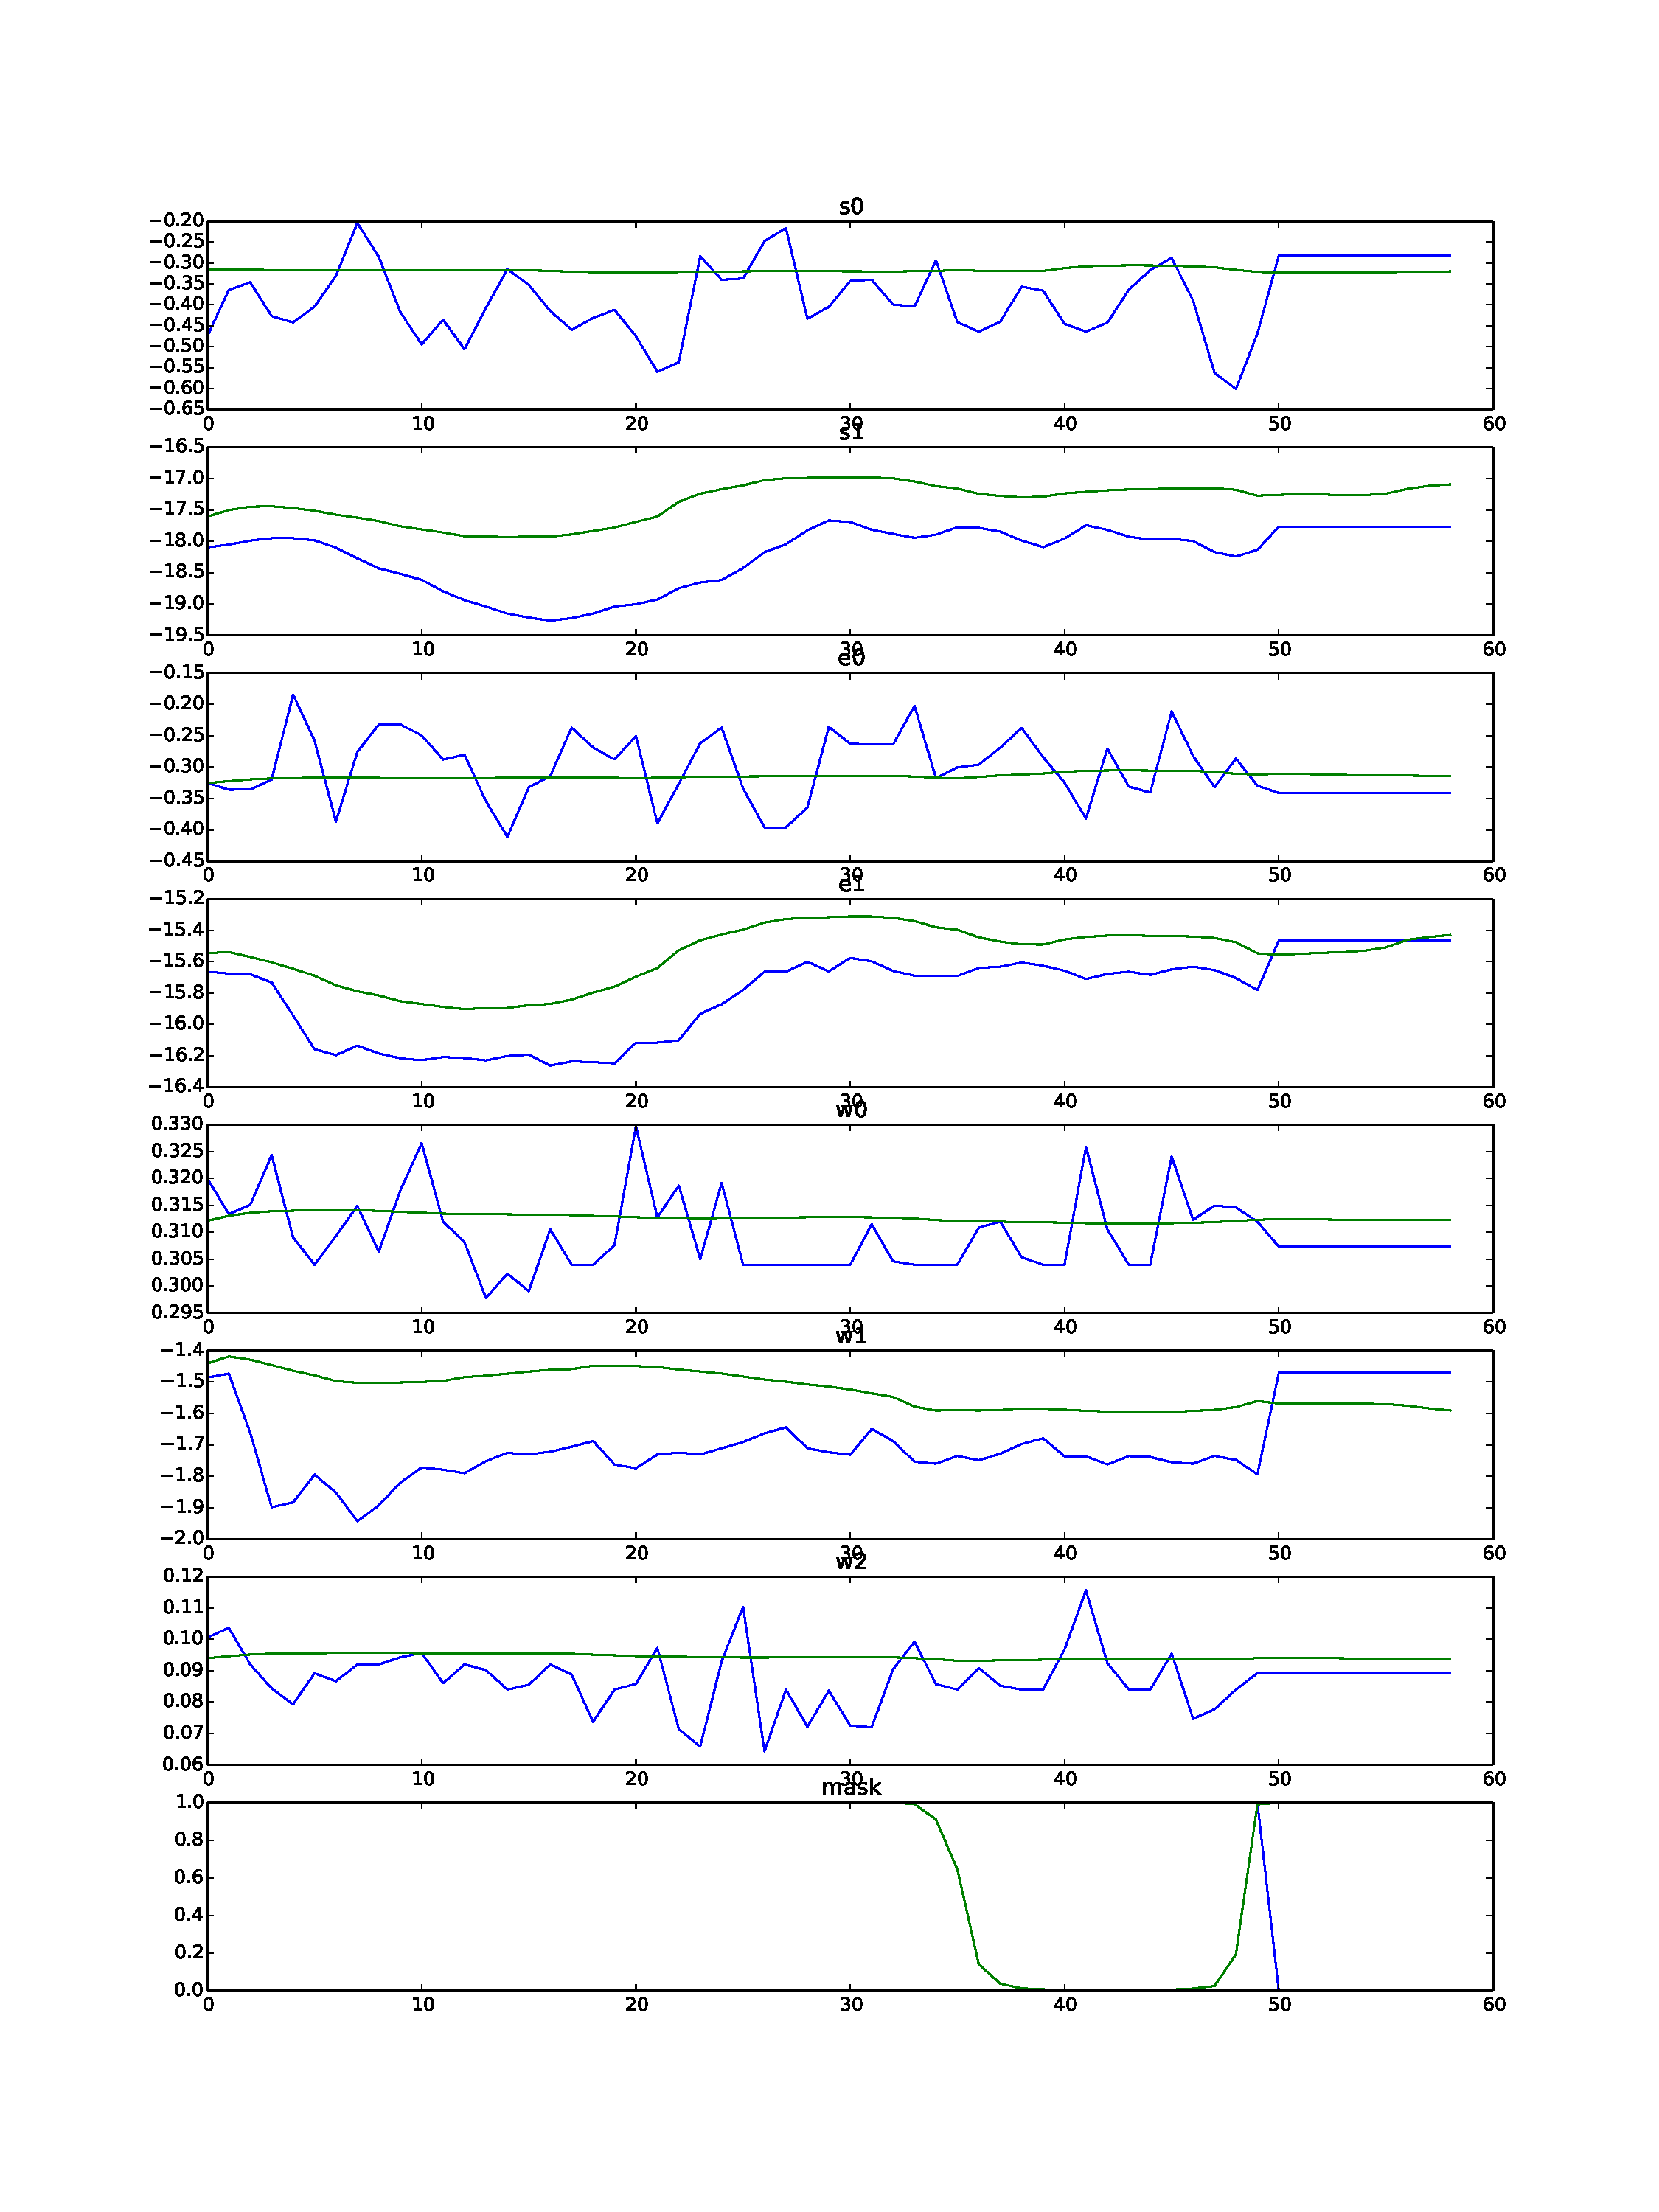
\includegraphics[width=\linewidth]{imagenes/resultados/pred_val.pdf}
		\caption{Validación}
		\label{fig:resultados/pred_val}
	\end{subfigure}
	\begin{subfigure}{0.3\textwidth}
		\centering
		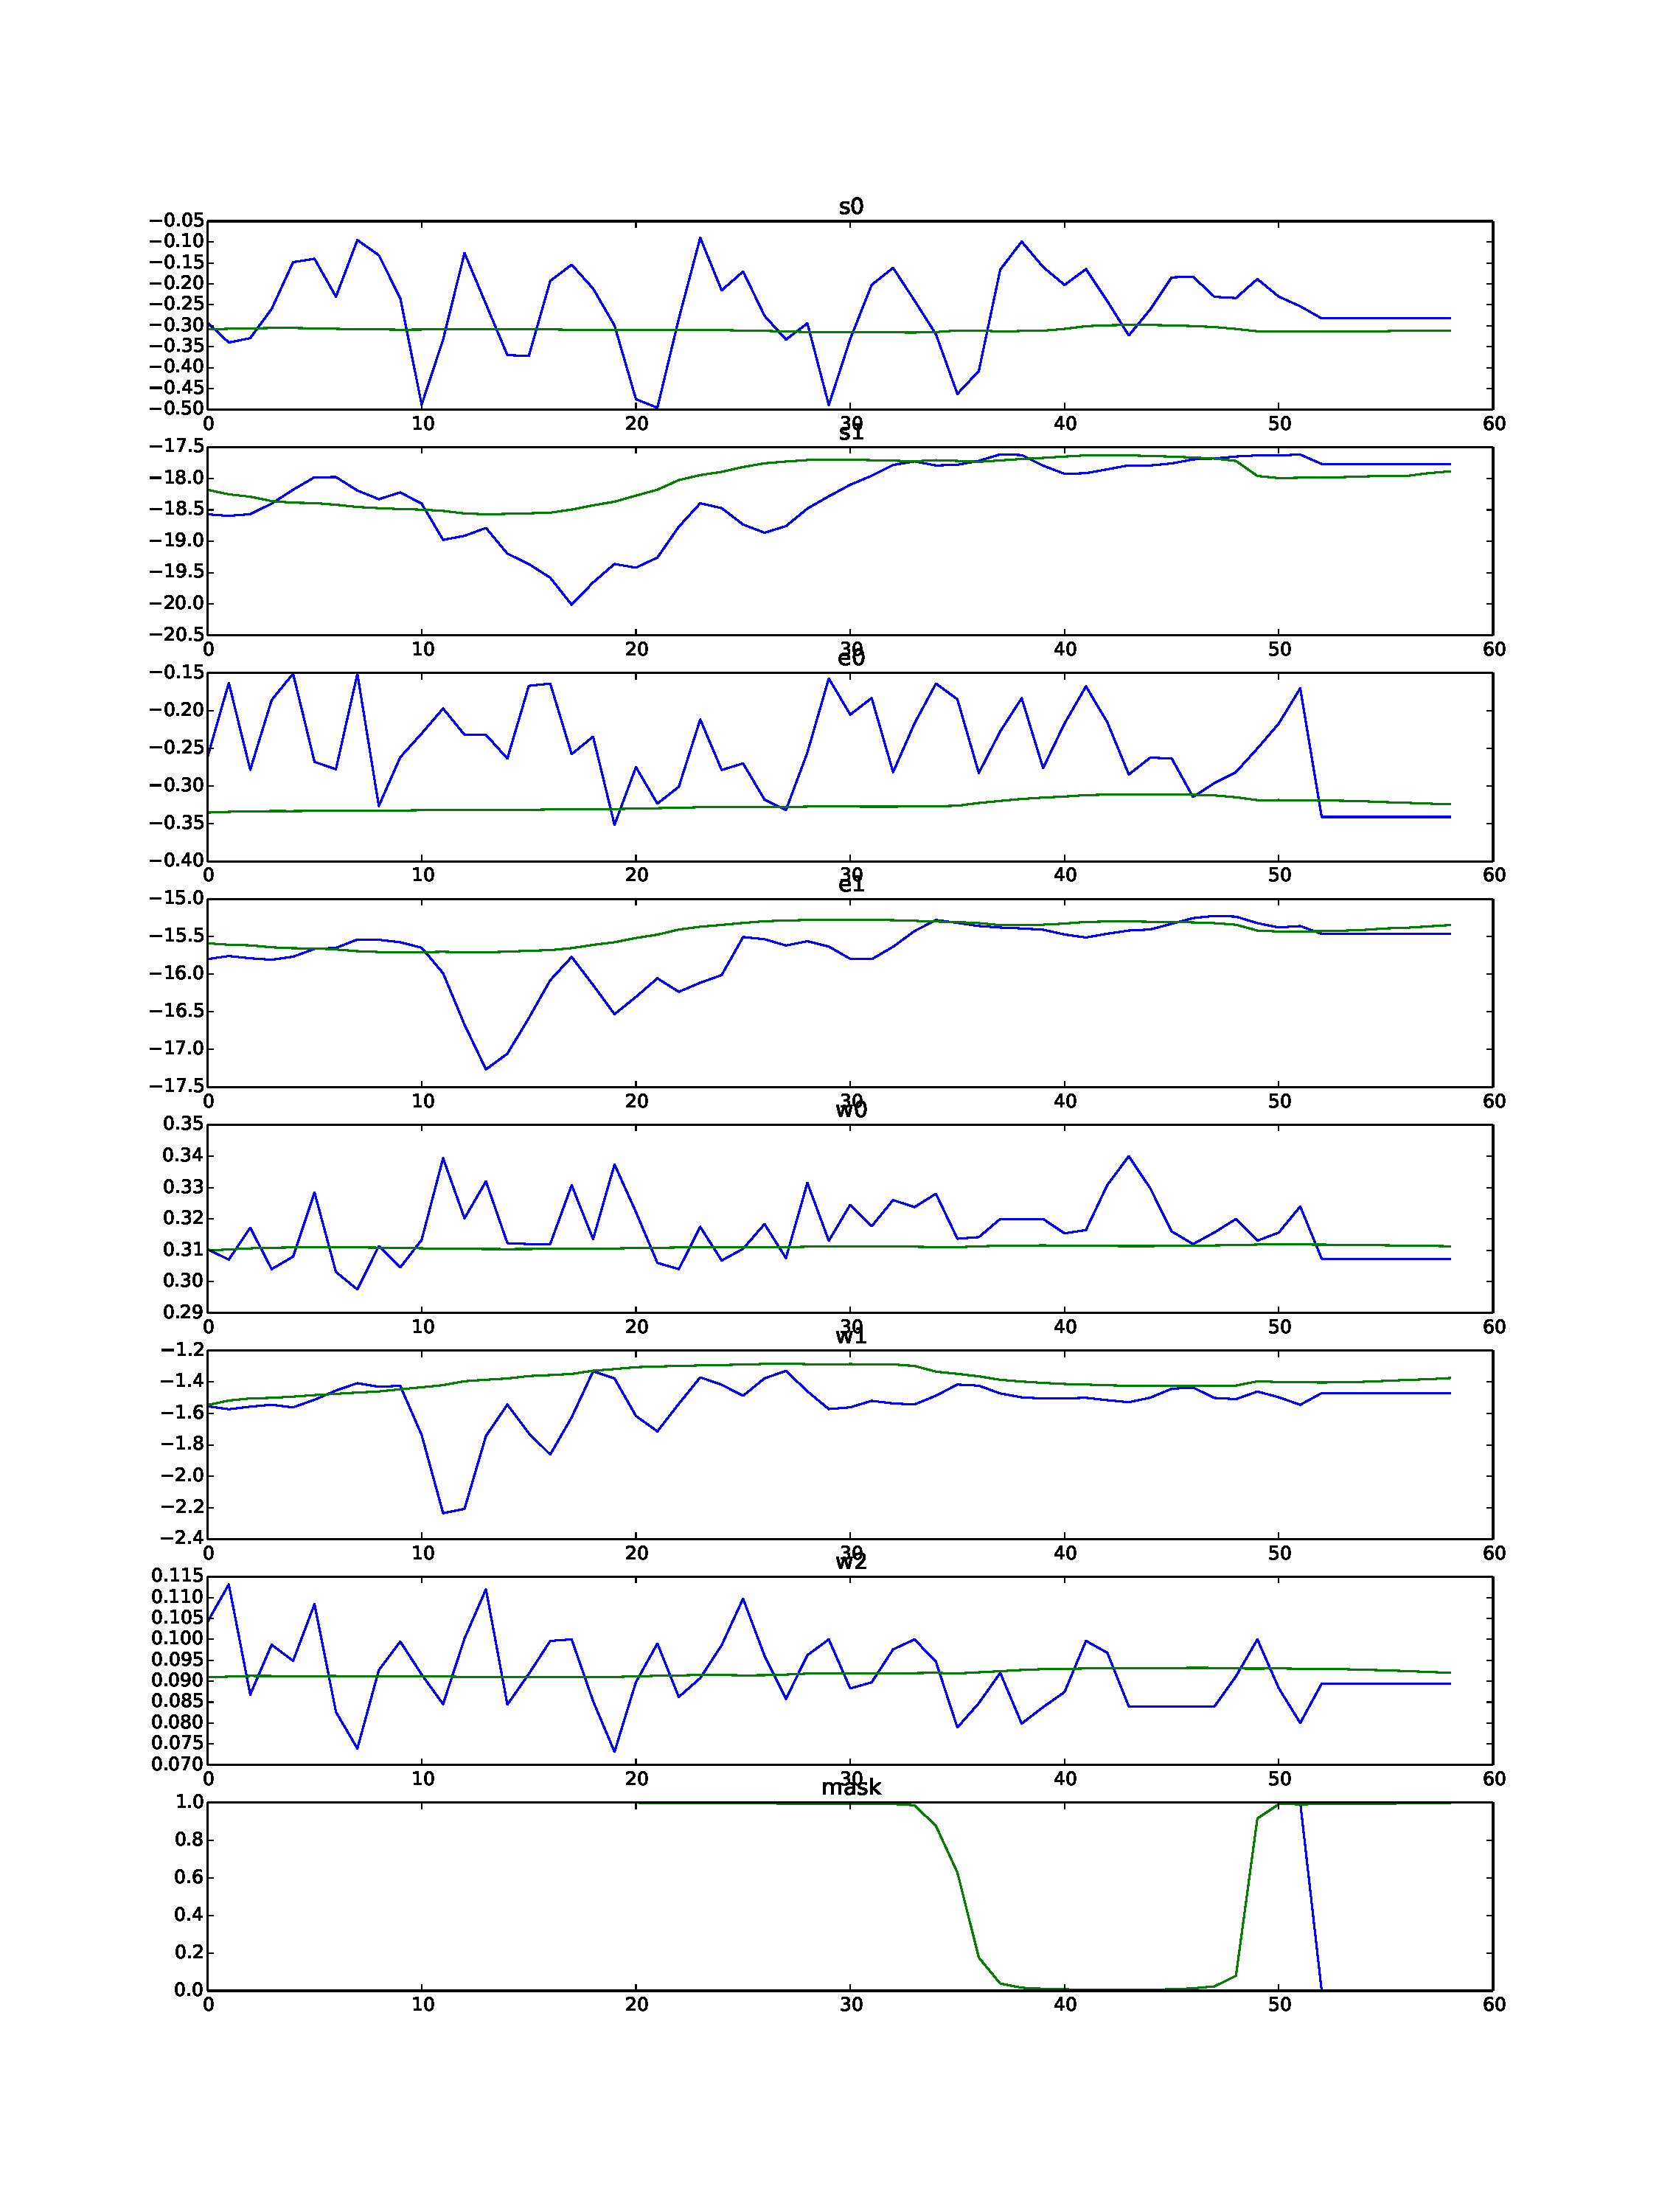
\includegraphics[width=\linewidth]{imagenes/resultados/pred_test.pdf}
		\caption{Test}
		\label{fig:resultados/pred_test}
	\end{subfigure}
	\caption{Errores en el torque}
	\label{fig:resultados/pred}
\end{figure}

